\documentclass[10pt]{article}
% Эта строка — комментарий, она не будет показана в выходном файле
\usepackage{ucs}
\usepackage[utf8x]{inputenc} % Включаем поддержку UTF8
\usepackage[russian]{babel}  % Включаем пакет для поддержки русского языка
\usepackage{amsmath}
\usepackage{amssymb}
\usepackage{mathtools}

\hoffset=0mm
\voffset=0mm
\textwidth=170mm        % ширина текста
\oddsidemargin=-0mm   % левое поле 25.4 - 5.4 = 20 мм
\textheight=240mm       % высота текста 297 (A4) - 40
\topmargin=-15.4mm      % верхнее поле (10мм)
\headheight=5mm      % место для колонтитула
\headsep=5mm          % отступ после колонтитула
\footskip=8mm         % отступ до нижнего колонтитула



% \textwidth=180mm    
% \oddsidemargin=-10mm 

\title{Работа 2.4. {\it Определение вязкости воздуха
по скорости течения через тонкие трубки.}}
\author{Зотов Алексей, 497}
\date{\today}

\begin{document}

\maketitle
\textbf{Цель работы:}
    \begin{enumerate}
    \item Экспериментально выявить участки ламинарного и турбулентного течения.
    \item Определить число Рейнольдса. 
    \item Определить вязкость воздуха.
    \item Экспериментально определить зависимость расхода воздуха в трубках от радиуса.
    \end{enumerate}
\textbf{В работе используются:} металлические трубки, укрепленные на горизонтальной подставке; газовый счетчик; микроманометр типа ММН; стеклянная U-образная трубка; секундомер.
\begin{center}
    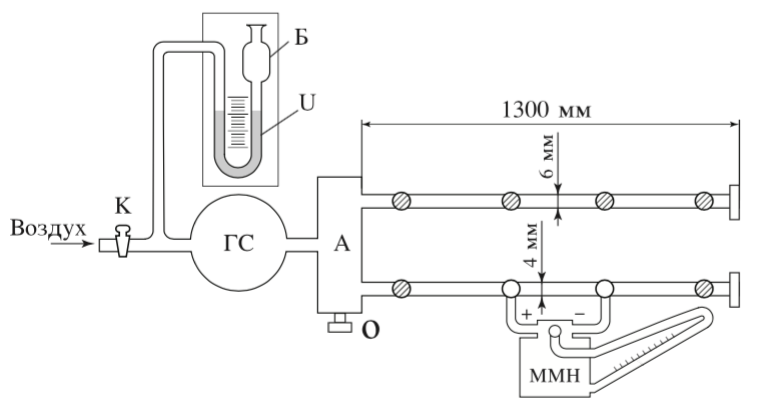
\includegraphics[width=8cm]{ust.png}
\end{center}

\textbf{Теоретическое введение.}
Если два соприкасающихся слоя газа текут с разной скоростью, то между ними возникает сила вязкого трения. Та же сила может действовать на твёрдые тела (по касательной к поверхности), помещённые в поток жидкости или газа. Причина возникновения этой силы заключается в следующем. Скорость частиц в текучей среде складывается из средней скорости потока и хаотической  — тепловой — составляющей. Следовательно, частицы могут перескакивать случайным образом из слоя в слой, перенося вместе с собой часть импульса потока из того слоя, откуда совершен скачок. Перенос же импульса от слоя к слою, согласно 2-му закону Ньютона, эквивалентен силовому взаимодействию между ними. Эта сила направлена по касательной к слоям, поскольку переносится компонента импульса, направленная вдоль среднего потока.Для количественного описания вязкого трения рассмотрим взаимодействие слоёв газа, текущего вдоль оси $x$, скорость потока которого изменяется в поперечном направлении $v_x = v_y(y)$ (см. рис. 1).

Пусть концентрация всюду одинакова и равна $n$, а средняя тепловая скорость хаотичного движения молекул равна$v_T$. Также для дальнейшего рассмотрения нам понадобится понятие длины свободного пробега $\lambda$
— среднего расстояния, которое пролетает молекула между столкновениями с другими молекулами.

Рассмотрим плоскость $y = 0$. Предположим, что через неё сверху вниз пролетают только молекулы, вылетевшие из слоя $0 < y < +\lambda$ (слой 2) и снизу вверх — вылетевшие из слоя $-\lambda < y < 0$ (слой 1). Данное предположение вполне разумно для качественной оценки явления, поскольку молекулы из более дальних слоёв имеют значительно меньшую вероятность добраться до $ y = 0$, поскольку по пути они скорее всего столкнутся с другими молекулами.

Количество молекул, перелетающих из слоя 1 в слой 2 за единицу времени через единичную площадку (плотность потока), равно:

\begin{equation}
        j = \frac{dN}{S \cdot dt} = \frac{1}{4} n v_t.
\end{equation}

Каждая из этих молекул массой $m_0$ обладает, помимо хаотично распределённой тепловой составляющей (в среднем $v_T$), дополнительной горизонтальной скоростью, связанной с движением в потоке $v_{1 x} = v_x(-\lambda)$, и горизонтальным импульсом $p_{1 x} = m_0 v_{1 x}$.
И наоборот, из слоя 2 в слой 1 поступает такое же количество молекул, но их средний горизонтальный импульс равен $p_{2 x} = m_0 c_{2 x}$. Горизонтальный импульс, который они переносят в сумме в единицу времени, и есть касательная сила вязкого трения:



$F_x = (\frac{dP_x}{dt})_{2 \to 1}  - (\frac{dP_x}{dt})_{1 \to 2} = j S (p_{2 x} - p_{1 x}) = S \cdot \frac{1}{4} m_0 n v_T \cdot (v_{2 x} - v_{1 x}).$



Считая $\lambda$ достаточно  малой,  раскладываем  по  Тэйлору $v_{2 x} - v_{1 x} = v_{x}(\lambda) - v_{x}(-\lambda)$, из чего получим окончательное
выражение для силы вязкого трения. В общем виде оно выглядит
следующим образом:

\begin{equation}
        F_x = S \eta \frac{d v_x}{dy}, 
\end{equation}

где $\eta$— коэффициент вязкости (сокращенно вязкость), $y$ — направление, перпендикулярное потоку, $S$ — площадь поверхности, для которой рассчитывается приложенная сила. В общих чертах механизм возникновения вязких сил трения во всех текучих средах (жидкостях и газах) одинаков, и формула (2) представляет собой определение
коэффициента вязкости.Для идеального газа, как следует из приведенных выше выкладок, вязкость можно оценить
по порядку величины:

\begin{equation}
        \eta \sim \frac{1}{2} m_0 n v_T \lambda = \frac{1}{2} \rho v_t \lambda, 
\end{equation}

Более детальное рассмотрение даёт значение вязкости, отли-
чающееся от полученного на множитель $\frac{2}{3}$. Хотя такое отличие не существенно для оценки по порядку величины, этот ответ является общепринятым для оценки $\eta$:

\begin{equation}
        \eta_ \sim \frac{1}{3} \rho v_t \lambda, 
\end{equation}

\textbf{Течение вязкой жидкости.}

Имеется два существенно различных класса течений. Ламинарное течение — течение, происходящее без перемешивания и пульсаций, в параллельных слоях жидкости; турбулентное течение, в котором образуются вихри и пульсации, а слои беспорядочно перемешиваются. 

То, каким будет данное конкретное течение, зависит от соотношения физических параметров и от геометрических характеристик системы. Если у системы есть характерный размер $r$ (радиус трубки при течении по трубе, радиус шарика при обтекании его внешним потоком и т. п.), то из $r$, плотности, вязкости $\eta$ и характерной скорости потока $v$ можно составить безразмерное соотношение:

\begin{equation}
        Re = \frac{\rho v r}{\eta}
\end{equation}
 
называемое числом Рейнольдса.
Безразмерные параметры отражают связь между физическими явлениями, происходящими на разных масштабах, и часто используются при описании сложных физических явлений, для которых нет точных решений. Величины $v, \rho, r, \eta$ могут меняться в широком диапазоне (например, течение воздуха в аэродинамической трубе диаметром в десятки метров и течение воды в капилляре), но если число $Re$ для этих случаев будет одинаково, то эти течения будут подобны друг другу. Такие зависимости в физике называют законами подобия.

Число Рейнольдса характеризует (по порядку величины) отношение кинетической энергии элемента жидкости к работе сил вязкого трения, совершаемой над ним. Действительно, кинетическая энергия в кубике со стороной $r$ равна
$ k \sim \frac{\rho r^3 v^2}{2}$, сила трения $F \sim \frac{r^2 \eta v}{r}$ и её работа $ A_F \sim F r \sim \eta v r^2 $, откуда

\begin{center}
    $Re \sim \frac{K}{A_F}$.
\end{center}
\small{
Вязкие силы стремятся стабилизировать течение, тогда как избыток кинетической энергии может приводить к переходу её части в вихревое движение. Таким образом, можно заключить, что большие числа Рейнольдса благоприятствуют рождению турбулентных течений, а при малых Re течение будет, скорее всего, ламинарным.}

Эксперимент подтверждает эти рассуждения: для заданной геометрии течения существует критическое значение числа Рейнольдса $Re_{\text{кр}}$, так что при $Re > Re_{\text{кр}}$ ламинарное течение оказывается неустойчивым и рождается турбулентность. Для течения по трубе эксперимент даёт $Re_{\text{кр}}\sim 10^3.$

\textbf{Течение по трубе.} Рассмотрим стационарное течение вязкой жидкости или газа по трубке круглого сечения радиуса $R$. Закон такого движения описывается формулами Пуазейля:
\begin{equation}
        v = \frac{P_1 - P_2}{L} \frac{1}{4 \eta} (R^2 - r^2),
\end{equation}
\begin{equation}
    Q = \frac{\pi R^4}{8 \eta L} (P_1 - P_2)
\end{equation}

где $P_2$ и $P_1$ — давления на концах трубы, а $L$ — длина трубы. \\ \\

\textbf{Ход работы:}

\begin{enumerate}

    \item  Будем снимать зависимость разности давлений $\bigtriangleup P$ на некотором участке трубы от расхода воздуха $\bigtriangleup Q = \frac{\bigtriangleup V}{\bigtriangleup t}$, при этом $\bigtriangleup V$ измеряется газовым счетчиком, а $\bigtriangleup t$— секундомером. Измерения будем проводить на участке с установившимся потоком (для трубки с диаметром 3.9 и 5.9мм возьмём участок длиной 50 см). Множитель на стойке микроманометра установим равным 0.2. Постепенно увеличим расход, начиная с маленьких перепадов давления.

    Найдем $k = \frac{\Delta P} {Q}$ как коэффициент наклона прямой$\Delta P(Q)$ на участке, соответствующему ламинарному течения. \\
    Получим $\eta$ из формулы Пуазейля(10):
    
    \begin{equation}
        \eta = \frac {\pi R ^ 4 \Delta P}{8 QL} = k \frac {\pi R ^ 4 }{8 L}
    \end{equation}
    
    Оценку $Re$ получим из следующих соотношений:

    \begin{equation}    
        Re = \frac{\rho vr}{\eta} = \frac{\rho lrS}{\eta tS} = \frac{\rho Q}{\eta \pi r}
    \end{equation}
    
    Относительную погрешность $\sigma_\eta$ определим из формулы:
    \begin{equation}
        \varepsilon_\eta^ 2 =  4^2 \varepsilon_r ^ 2 +  \varepsilon_{k} ^ 2 + \varepsilon_L ^ 2
    \end{equation}
    
    \begin{equation}    
        \varepsilon_k = \frac{1}{\sqrt{m-1}} \varepsilon_{k_{i}} = \frac{1}{\sqrt{m-1}} \sqrt{\varepsilon_{\Delta P}^2 + \varepsilon_{Q}^2}
        \text{, где } m \text{ - количество точек на участке ламинарного течения}
    \end{equation}          
    \underline{Погрешности измерения:}\\
    $\sigma_d = 0.05 $ мм \\
    $\sigma_V = 0.01  \text{дм}^3$  \\
    $\sigma_T = 0.5$с \\

    
                    % \begin{table}[h]
                    \begin{center}
                    $\Delta P (Q)$ , $d = 3.9$мм
                    \begin{tabular}{|c|c|c|c|c|c|c|c|c|c|c|}
                            \hline
                                $\Delta T , c$ & 67.9& 41.1& 22.2& 39.1& 18.9& 25.4& 21.2& 19.4& 17.5& 14.7 \\
                            \hline
                                 $\Delta V , m^3 * 10^{-3}$   & 0.3& 1.0& 1.0& 2.5& 1.5& 2.5& 2.5& 2.5& 2.5& 2.5 \\
                            \hline
                                $Q , m^3/s * 10^{-5}$ &0.442&2.433&4.513&6.395&7.949&9.839&11.815&12.92&14.286&17.053\\
                            \hline
                                $\Delta P , \text{Па}$ &7.845&33.343&60.801&84.337&107.873&154.945&245.166&302.045&360.885&519.752\\
                            \hline
                        \end{tabular}
                        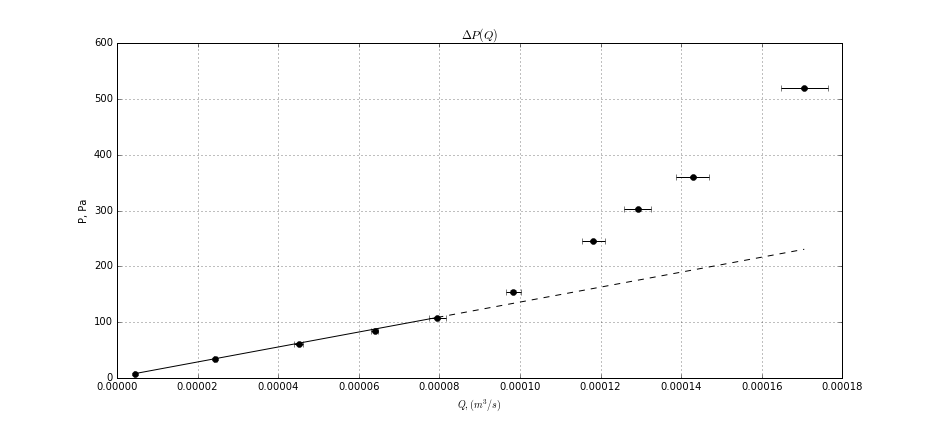
\includegraphics[width=15cm]{g1mm.png}
                    \\ Рис. 1: График зависимости разности давлений от расхода в трубке 1 ($d = 3.9$мм).
                    \end{center}
                    % \end{table}

            \begin{table}[h]
                    \begin{center}
                    $\Delta P (Q)$ , $d = 5.9$мм\\
                    \begin{tabular}{|c|c|c|c|c|c|c|c|c|c|c|}
                            \hline
                                $\Delta T , c$ & 42.2& 27.3& 16.7& 13.8& 19.7& 17.3\\
                            \hline
                                 $\Delta V , m^3 * 10^{-3}$  & 1.0& 2.5& 3.0& 3.0& 5.0& 5.0\\
                            \hline
                                $Q , m^3/s * 10^{-5}$ &2.367&9.154&17.986&21.708&25.355&28.868\\
                            \hline
                                $\Delta P , \text{Па}$ &7.845&29.42&94.144&137.293&182.404&229.476\\
                            \hline
                            \end{tabular}
                        
                            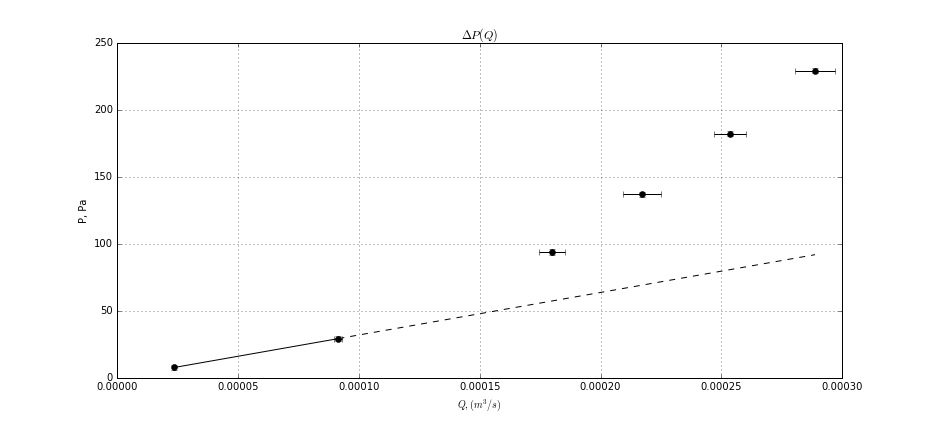
\includegraphics[width=15cm]{g2mm.png}
                            \\ Рис. 2: График зависимости разности давлений от расхода в трубке 2($d = 5.9$мм).
                    \end{center}
                    \end{table}
    \underline{Для $d = 3.9$мм:}
        \indent $m = 5$ - как видно из графика, 6-я точка уже немного отклоняется от на начальной прямой. Можно предположить, что нарушение ламинарного течения происходит между 5 и 6 точкой. \\
        \indent $k = 13.41 * 10^{-5} \frac{\text{Па}\cdot c}{\text{м}^3}$ , $\varepsilon_k = 0.037$ \\
        \indent $\varepsilon_{\eta} = 0.063$ \\
        \indent $\eta = (1.52 \pm 0.1) * 10^{-5}$ Па*с \\
        \indent $Re_{\text{кр}} \sim  930$ (взяв расход $ Q = (Q_5 + Q_6)/2$)
        \\ \\
    \underline{Для $d = 5.9$мм:}
        
        \indent $m = 2$ - уже первые 3 точки не лежат на прямой, можно сделать предположение что на участке от 1 до 2 течение ламинарное, а между 2 и 3 ламинарность нарушается. \\
        \indent $k = 3.18 * 10^{-5} \frac{\text{Па}\cdot c}{\text{м}^3}$ , $\varepsilon_k = 0.10$ \\
        \indent $\varepsilon_{\eta} =  0.11$ \\
        \indent $\eta = (1.89 \pm 0.21) * 10^{-5}$ Па*с \\
        \indent $Re_{\text{кр}} \sim  937$  (взяв расход $Q = (Q_2 + Q_3)/2$), получили значение близкое к полученному для тонкой трубки, что может говорить о правильности предположения длины участка ламинарного течения.
     
     \item Теоретическая вязкость при $\lambda \sim 10^{-5}$см: 
        \begin{equation}
                \eta_{th} = \frac{1}{3} \rho v_T \lambda = \frac{1}{3} \rho \lambda \sqrt{\frac{3RT}{m_{mol}}} \approx  2.02 \cdot 10^{-5} \text{Па с}
        \end{equation}
        где $m_{mol} \approx 28.98$г/моль - молярная масса воздуха
        
    Также в таблицах можно найти значение вязкости воздуха для $T \sim 15 - 20^o C:$

    $\eta_{table} = 1.86 \cdot 10^{-5} \text{Па с}$

    Полученные оптным путем и теретические значения совпадают в пределах погрешности. 
     
     \pagebreak
    \item Найдем зависимость $P$ от длины для трубок диаметром 3.9см и 5.9см при малом давлении
                    % \begin{table}[h]
                    \begin{center}
                    $d = 3.9$мм , $Q = 0.042 \text{дм}^3/\text{c}$

                    \begin{tabular}{|c|c|c|c|c|}
                            \hline
                                $x ,$ м  &0.105&0.405&0.805&1.305\\
                            \hline
                                $P(x) , \text{Па}$ &27.5&66.7&107.9&164.8\\
                            \hline
                        \end{tabular}
                        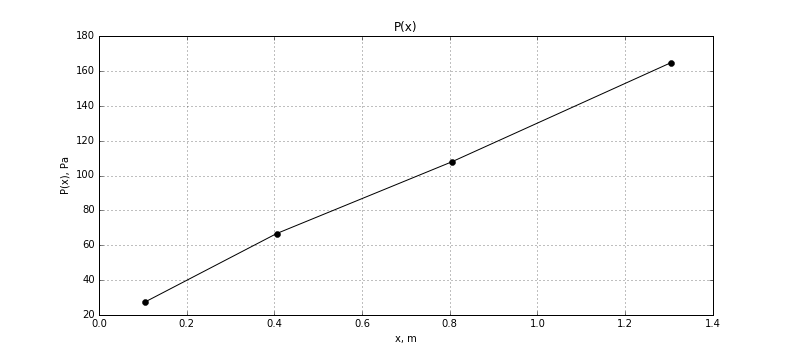
\includegraphics[width=15cm]{g11mm.png}
                    \\ Рис. 3: График распределения давления от координаты $x$.\\
                    
                    Как видно из графика, коэффициент наклона на участке [0.1:0.4] отличается от коэффициента наклона на последующих участках: $L_\text{установления} \in (0.1,0.4)$ м 


                    $d = 5.9$мм, $Q = 0.084 \text{дм}^3/\text{c}$

                    \begin{tabular}{|c|c|c|c|c|}
                            \hline
                                $x ,$ м  &0.105&0.405&0.805&1.305\\
                            \hline
                                $P(x) , \text{Па}$ &23.5&39.2&60.8&88.3\\
                            \hline
                        \end{tabular}
                        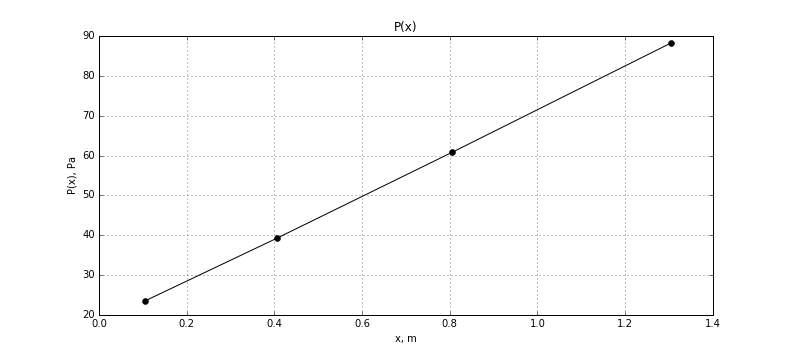
\includegraphics[width=15cm]{g22mm.png}
                    \\ Рис. 4: График распределения давления координаты $x$. 
                    \\График линеен на измеренном участке, значит $L_\text{установления} \leq 0.1$ м.                    
                    \end{center}
                    % \end{table}


\end{enumerate}
\end{document}


